% begin module sequence-ex7
\begin{frame}
\begin{example}[Example 7, p. 716]
Is $a_n = \frac{(-1)^n}{n}$ convergent or divergent?
\begin{columns}[c]
\column{.5\textwidth}
\ \only<handout:0| -4>{%
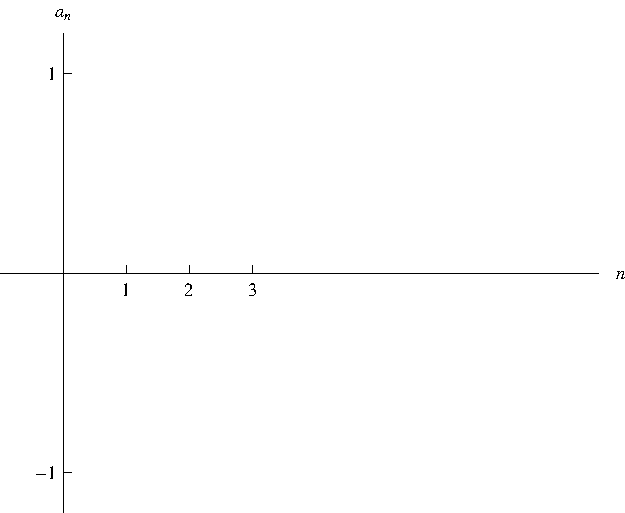
\includegraphics[height=4cm]{sequences/pictures/12-01-ex7a.pdf}%
}%
\only<5->{%
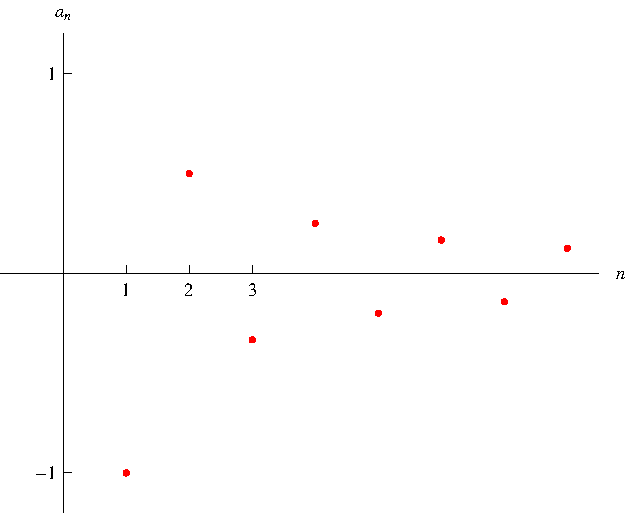
\includegraphics[height=4cm]{sequences/pictures/12-01-ex7b.pdf}%
}%
\column{.5\textwidth}
\[
\uncover<2->{%
\lim_{n\to\infty}\left| \frac{(-1)^n}{n}\right| = %
}%
\uncover<3->{%
\lim_{n\to\infty} \frac{1}{n} = %
}%
\uncover<4->{%
0%
}%
\]
\uncover<5->{%
Therefore, by the corollary to the Squeeze Theorem,
\[
\lim_{n\to\infty}\frac{(-1)^n}{n} = 0%
\]
}%
\uncover<6->{%
Therefore $\left\{ \frac{(-1)^n}{n} \right\}$ is convergent.
}%
\end{columns}
\end{example}
\end{frame}
% end module sequence-ex7
